\section{Utilisation de bibliothèques}

En python, il existe de nombreuses manières de produire des graphiques. 
Pour ce faire, nous allons utiliser la bibliothèque \texttt{matplotlib.pyplot}. 

Une bibliothèque est un regroupement de fonctions, livrées directement avec Python\ ou écrites par un tiers.
Nous allons en utiliser plusieurs cette année : 
\begin{itemize}
  \item \texttt{math}, pour utiliser des fonctions mathématiques de base ; 
  \item \texttt{random}, pour simuler des expériences aléatoires ; 
  \item \texttt{time}, pour disposer d'un chronomètre ;
  \item \texttt{scipy.optimize}, pour résoudre certains problèmes numériques ; 
  \item \texttt{scipy.integrate} pour résoudre d'autres problèmes numériques ;
  \item \texttt{numpy}, pour utiliser des outils de calcul vectoriel ; 
  \item et donc \texttt{matplotlib.pyplot}, pour avoir des outils de tracé graphique. 
\end{itemize}
Certaines de ces bibliothèques sont toujours disponibles avec Python, comme les bibliothèques \texttt{math} et \texttt{random}, elles font partie de la bibliothèque standard. 
D'autres doivent être installées séparément, comme la bibliothèque \texttt{matplotlib.pyplot}, notamment. 

On charge une bibliothèque avec le mot clef \pyv{import}. Il existe plusieurs manières de charger une bibliothèque. Prenons l'exemple de la bibliothèque \texttt{math}.

On peut d'abord charger l'intégralité de la bibliothèque.
\begin{exemple}~
\begin{pyconsole}
import math
math.sqrt(2)
\end{pyconsole}
\end{exemple}
Remarquez qu'il est alors obligatoire de rappeler de quelle bibliothèque vient chaque commande (plusieurs bibliothèques peuvent proposer des implémentations différentes d'une même fonction).
\begin{exemple}
La fonction \texttt{exp} du module \texttt{math} ne s'applique qu'à des nombres flottants, alors que celle de \texttt{numpy} peut s'appliquer à des vecteurs (cette structure sera détaillée ultérieurement). 
\begin{pyconsole}
import numpy
math.exp(1)
numpy.exp(1)
numpy.exp([1,2,3])
\end{pyconsole}
\end{exemple}
On peut donner un alias à une bibliothèque avec le mot clef \pyv{as}, afin de pouvoir l'utiliser rapidement. 
\begin{exemple}~
\begin{pyconsole}
import math as m
m.pi
\end{pyconsole}
\end{exemple}
On peut aussi décider de n'importer que certaines fonctions d'une bibliothèque, avec le mot clef \pyv{from}. Dans ce cas, on peut utiliser la fonction importée sans préfixe. 
\begin{exemple}~
\begin{pyconsole}
from math import log
log(2)
\end{pyconsole}
\end{exemple}
On peut aussi importer toutes les fonctions d'un coup de cette manière, en utilisant le joker \texttt{*}.
\begin{exemple}~
\begin{pyconsole}
from math import *
tan(pi/4)
\end{pyconsole}
\end{exemple}

\section{Matplotlib.pyplot}

La bibliothèque \texttt{matplotlib.pyplot} fournit des outils de tracés graphiques très proches de ceux du logiciel Matlab. 
On essaiera toujours de l'utiliser de la manière suivante. 
\begin{enumerate}
  \item Appeler la fonction \texttt{clf()} (pour \emph{clean figure}) pour effacer la figure précédente, et donc en commencer une nouvelle. 
  \item Tracer des courbes, nuages de points, en appelant (éventuellement plusieurs fois) la fonction \texttt{plot()}. On remarquera que rien n'est ici affiché : seul un objet est créé par Python. 
  \item Éventuellement, paramétrer le graphique (axes, titre, légendes \emph{etc.}) en utilisant les fonctions adéquates. 
  \item Afficher le graphique avec la fonction \texttt{show()} ou, mieux, le sauvegarder avec la fonction \texttt{savefig()}. On dispose alors d'une image (différents formats possibles). 
\end{enumerate}

\section{Utilisation de la fonction \texttt{plot}}

Cette fonction peut-être utilisée de nombreuses manières différentes, pour obtenir des résultats assez fins. Nous ne les 
détaillerons pas toutes ici. 
L'idée générale est de lui donner en argument deux tableaux de nombres, décrivant respectivement les abscisses et les ordonnées des points à tracer. 
Sans autre option, ces points sont reliés par des segments bleus, en traits pleins. 
\begin{exemple}
  Le code suivant produit la figure~\ref{fig:ex_base_01}.
% Fichier ex_base_01.py
\begin{pyverbatim}
import matplotlib.pyplot as plt

x = [1, 3, 4, 2]
y = [2, 1, 4, 2]

plt.clf()
plt.plot(x,y)
plt.savefig("ex_base_01.png")
\end{pyverbatim}


%\begin{figure}[!h]
  \begin{center}
  \begin{tabular}{c}
    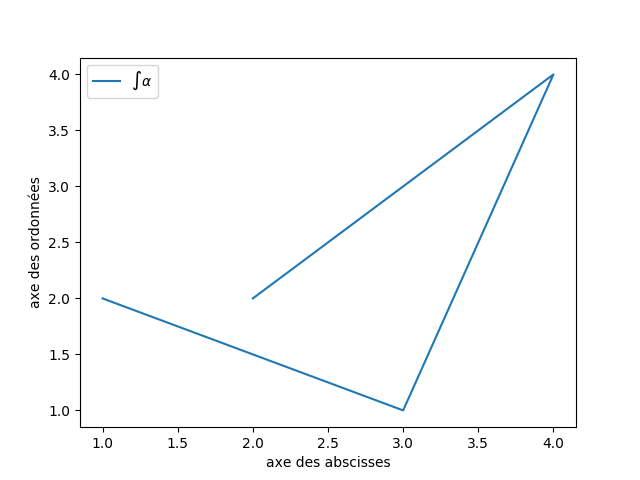
\includegraphics[scale = 0.5]{ex_base_01} \\
    \end{tabular}
  \captionof{figure}{Style standard}
    \label{fig:ex_base_01}
  \end{center}
%\end{figure}
\end{exemple}

Les options graphiques permettent notamment de modifier le type de segment (pointillés, sans segment), d'afficher ou non un marqueur au niveau de chaque point et de changer la couleur de ces objets. 
\begin{exemple}
  Le code suivant produit la figure~\ref{fig:ex_base_02}.
% Fichier ex_base_02.py
\begin{pyverbatim}
import matplotlib.pyplot as plt

x = [1, 3, 4, 2]
y = [2, 1, 4, 2]

plt.clf()
plt.plot(x,y,'or--')
plt.savefig("ex_base_02.png")
\end{pyverbatim}
%\begin{figure}[!h]
  \begin{center}
    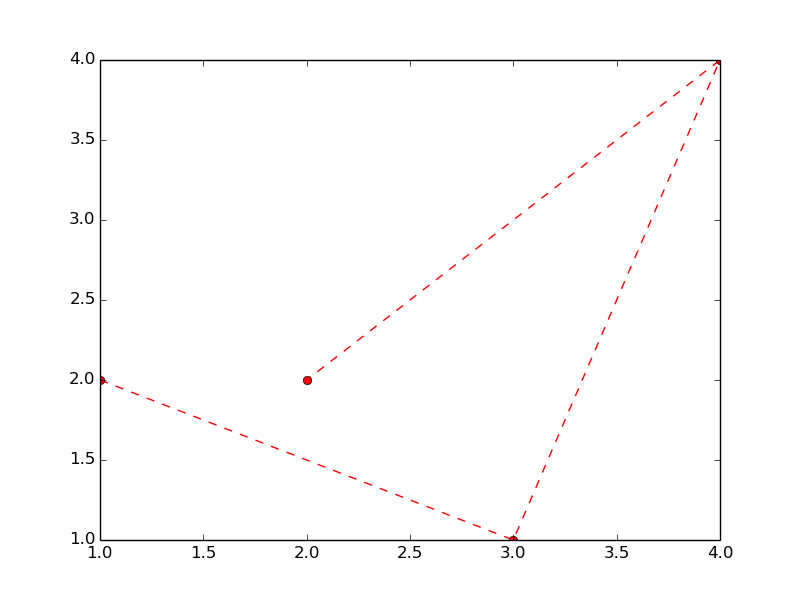
\includegraphics[scale = 0.5]{ex_base_02}
    \captionof{figure}{Points marqués, ligne coupée, couleur rouge.}
    \label{fig:ex_base_02}
  \end{center}
%\end{figure}
On remarquera que cette figure aurait aussi pu être obtenue par la commande suivante, plus explicite mais moins concise. 
% Fichier ex_base_02.py
\begin{pyverbatim}
plt.plot(x,y,marker='o',color='r',linestyle='--')
\end{pyverbatim}
\end{exemple}

On peut enfin appeler plusieurs fois la fonction \texttt{plot} successivement. Les tracés sont alors superposés. 
\begin{exemple}
  Le code suivant produit la figure~\ref{fig:ex_base_03}.
% Fichier ex_base_03.py
\begin{pyverbatim}
import matplotlib.pyplot as plt

x = [1.5, 3, 3.5, 2]
y = [3, 2, 4, 2]

plt.clf()
plt.plot(x,y,'or')
plt.plot([1,4],[1,4])
plt.savefig("ex_base_03.png")
\end{pyverbatim}
%\begin{figure}[!h]
  \begin{center}
    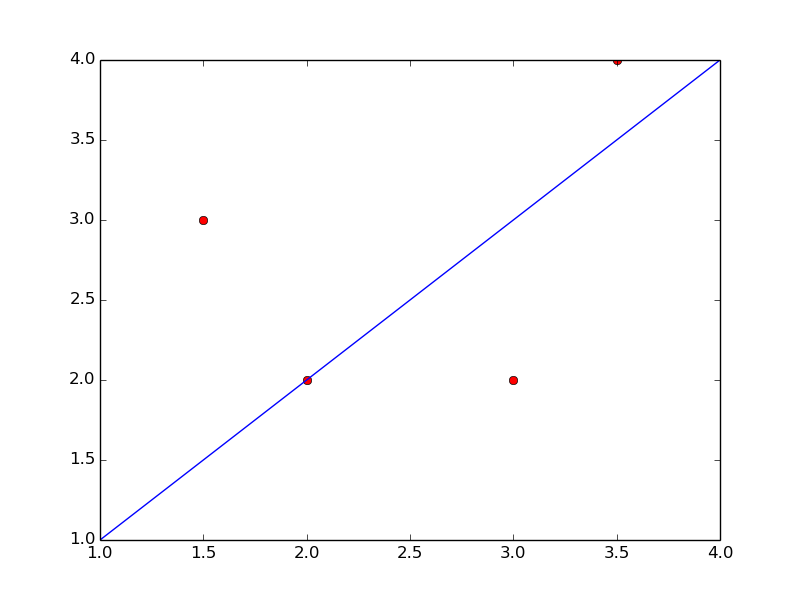
\includegraphics[scale = 0.5]{ex_base_03}
    \captionof{figure}{Supperposition de deux tracés}
    \label{fig:ex_base_03}
  \end{center}
%\end{figure}
\end{exemple}
\begin{rem}
  Il n'est pas réellement possible de tracer des courbes lisses, mais seulement des lignes brisées et des nuages de 
points. 
\end{rem}


\section{Quelques options graphiques disponibles}

La fonction \texttt{plot()} possède énormément d'options, nous n'en détaillerons que quelques-unes ici. On suppose dans 
cette partie que la bibliothèque \texttt{matplotlib.pyplot} a été importée avec l'alias \texttt{plt}.

\subsection{Couleurs (option \texttt{color})}

On peut décrire de nombreuses couleurs très précisément, mais certaines sont disponibles avec les raccourcis suivants. 
L'argument donné est une chaîne de caractères et la couleur par défaut est le bleu. 

\begin{table}[!h]
  \begin{center}
    \begin{tabular}{|c|c|}
      \hline
      Mot clef & Couleur \\
      \hline 
      \texttt{'b'} & Bleu \\
      \hline 
      \texttt{'g'} & Vert \\
      \hline 
      \texttt{'r'} & Rouge \\
      \hline 
      \texttt{'c'} & Cyan \\
      \hline 
      \texttt{'m'} & Magenta \\
      \hline 
      \texttt{'y'} & Jaune \\
      \hline 
      \texttt{'k'} & Noir \\
      \hline 
      \texttt{'w'} & Blanc \\
      \hline
    \end{tabular}
    \caption{Couleurs prédéfinies dans \texttt{matplotlib}.}
  \end{center}
\end{table}
\begin{exemple}
  Pour tracer une courbe en magenta, on écrira la commande suivante.
\begin{pyverbatim}
plt.plot(x,y,color = 'm')
\end{pyverbatim}
\end{exemple}

\subsection{Étiquette (option \texttt{label})}


On peut adjoindre à un tracé une chaîne de caractères (son étiquette), qui pourra notamment être utilisée dans les légendes. 
Les parties entres deux symboles \$ sont interprétées comme du code LaTeX  (attention, en Python, le caractère \textbackslash\ se code par le caractère \texttt{'\textbackslash\textbackslash'}). 
Par défaut, il n'y a pas d'étiquette.
\begin{exemple}
  Pour donner le nom \og $\arccos(t)$ \fg\ à la courbe, on écrira la commande suivante.
\begin{pyverbatim}
plt.plot(x,y,label = '$\\arccos(t)$')
\end{pyverbatim}
\end{exemple}
\subsection{Type de ligne (option \texttt{linestyle})}

On peut spécifier plusieurs types de lignes, qui seront utilisés pour tracer les segments reliant les points donnés en argument. 
L'argument donné est une chaîne de caractères et, par défaut, la ligne est tracée continuement. 

\begin{table}[!h]
  \begin{center}
    \begin{tabular}{|c|c|}
      \hline
      Mot clef & Type de ligne \\
      \hline
      \texttt{'-'} & Ligne continue \\
      \hline
      \texttt{'- -'} & Tirets  \\
      \hline
      \texttt{'-.'} & Alterne tirets et points \\
      \hline
      \texttt{':'} & Ligne pointillée \\
      \hline
      \texttt{'None'} ou \texttt{' '} ou \texttt{''} & Pas de ligne \\
      \hline
    \end{tabular}
    \caption{Types de ligne disponibles.}
  \end{center}
\end{table}

\begin{exemple}
  Pour tracer une courbe en pointillés, on écrira la commande suivante.
\begin{pyverbatim}
plt.plot(x,y,linestyle = ':')
\end{pyverbatim}
\end{exemple}

\subsection{Épaisseur des lignes (option \texttt{linewidth})}

On peut régler l'épaisseur des lignes reliant les points.
L'argument donné est un flottant, qui vaut 1 par défaut. 

\begin{exemple}
  Pour tracer une courbe dont le trait est deux fois plus épais que la normale, on écrira la commande suivante.
\begin{pyverbatim}
plt.plot(x,y,linewidth = 2)
\end{pyverbatim}
\end{exemple}

\subsection{Type de point (option \texttt{marker})}

On peut changer la manière dont les points sont représentés. 
L'argument donné est une chaîne de caractères et, par défaut, les points ne sont pas représentés. 

\begin{rem}
  La liste donnée dans la table~\ref{tab:marker} est loin d'être exhaustive. 
\end{rem}


\begin{table}[!h]
  \begin{center}
    \begin{tabular}{|c|c|}
      \hline
      Mot clef & Type de point \\
      \hline
      \texttt{'.'} & Point \\
      \hline
      \texttt{'o'} & Cercle \\
      \hline
      \texttt{'s'} & Carré \\
      \hline
      \texttt{'*'} & Étoile \\
      \hline
      \texttt{'+'} & Croix (forme $+$) \\
      \hline
      \texttt{'x'} & Croix (forme $\times$) \\
      \hline
      \texttt{'None'} ou \texttt{' '} ou \texttt{''} & Pas de point \\
      \hline
      \texttt{'\$...\$'} & Texte Latex (à la place de ...) \\
      \hline
    \end{tabular}
    \caption{Quelques types de points disponibles.}
    \label{tab:marker}
  \end{center}
\end{table}

\begin{exemple}
  Pour placer des carrés à l'emplacement des points indiqués, on écrira la commande suivante.
\begin{pyverbatim}
plt.plot(x,y,marker = 's')
\end{pyverbatim}
\end{exemple}

\begin{rem}
  Les options \texttt{markeredgecolor}, \texttt{markeredgwidth}, \texttt{markerfacecolor} et \texttt{markersize} permettent de paramétrer plus finement l'apparence des points. 
\end{rem}

\section{Autres fonctions utiles}

Nous avons déjà vu comment utiliser de manière élémentaire les fonctions \texttt{clf()}, \texttt{plot()} et \texttt{savefig()}.

\subsection{Paramètres avancés d'un graphique}

On peut affecter une étiquette à chaque axe avec les fonctions \texttt{xlabel()} et \texttt{ylabel()}.

Les fonctions \texttt{xlim()} et \texttt{ylim()} permettent de régler manuellement les étendues des deux axes, et donc la forme du graphique. On pourra utiliser à la place la fonction \texttt{axis()}.
On pourra aussi utiliser la fonction \texttt{autoscale()}.
Les fonctions \texttt{xticks()} et \texttt{yticks()} permettent de régler les graduations des axes. 

La fonction \texttt{figtext()} permet d'écrire du texte dans une figure. 

La fonction \texttt{legend()} permet d'ajouter une légende à une figure, la fonction \texttt{title()} permet d'ajouter un titre à une figure. 

Les commandes \texttt{xscale('log')} et \texttt{yscale('log')} permettent de passer les axes des abscisses ou des ordonnées en échelle logarithmique. 

\subsection{Quelques outils utiles en statistiques}

\emph{Cette partie ne sera pas utilisée en informatique, mais pourra vous intéresser dans le cadre de votre TIPE, notamment.}

Les fonctions \texttt{barh()} et \texttt{hist()} permettent de réaliser des histogrammes, la fonction \texttt{boxplot()} permet de réaliser des diagrammes en boîtes à moustaches.

La fonction \texttt{errorbar()} permet de tracer un graphe avec des barres d'erreurs (intervalles de confiances). 

\subsection{Subdivision régulière d'un intervalle}

Pour tracer une fonction, on trace en fait des cordes de cette fonction, à partir d'une subdivision de l'intervalle considéré. 
La fonction \texttt{linespace()} de la bibliothèque \texttt{numpy} permet de créer automatiquement de telles subdivisions, avec un nombre de points à régler manuellement. 

\begin{exemple}
Pour tracer le graphe de la fonction $x\mapsto x^3$ sur $[0,1]$ avec une subdivision en 3 segments, donc en utilisant 
4 points, on peut utiliser le code suivant, qui donne la figure~\ref{fig:ex_numpy_01}.
% Code du fichier ex_numpy_01.py
\begin{pyverbatim}
import matplotlib.pyplot as plt
from numpy import linspace

x = linspace(0,1,4)
y = [t**3 for t in x]

plt.clf()
plt.plot(x,y)
plt.xlabel('$t$')
plt.ylabel('$t^3$')
plt.savefig('ex_numpy_01.png')
\end{pyverbatim}

%\begin{figure}[!h]
  \begin{center}
    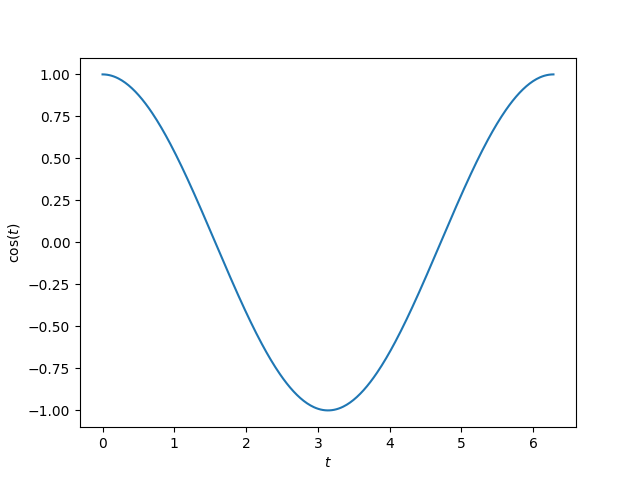
\includegraphics[scale = 0.5]{ex_numpy_01}
    \captionof{figure}{Subdivision en 3 segments}
    \label{fig:ex_numpy_01}
  \end{center}
%\end{figure}  
Pour obtenir une courbe plus lisse, on peut utiliser une subdivision plus fine. Par exemple, avec 100 segments, et donc 101 points, on peut utiliser le code suivant, qui donne la figure~\ref{fig:ex_numpy_02}.
% Code du fichier ex_numpy_01.py
\begin{pyverbatim}
import matplotlib.pyplot as plt
from numpy import linspace

x = linspace(0,1,101)
y = [t**3 for t in x]

plt.clf()
plt.plot(x,y)
plt.xlabel('$t$')
plt.ylabel('$t^3$')
plt.savefig('ex_numpy_01.png')
\end{pyverbatim}

%\begin{figure}[!h]
  \begin{center}
    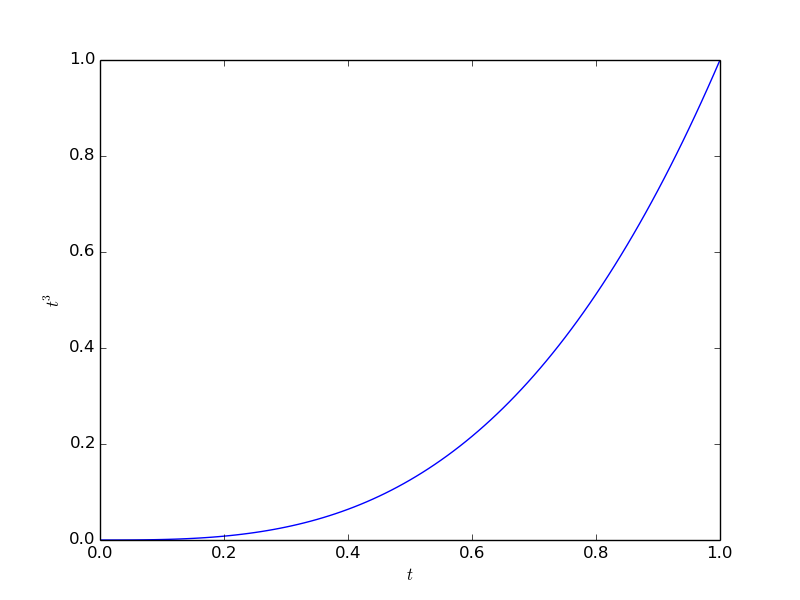
\includegraphics[scale = 0.5]{ex_numpy_02}
    \captionof{figure}{Subdivision en 100 segments}
    \label{fig:ex_numpy_02}
  \end{center}
%\end{figure}  
\end{exemple}


%\section{Exemple avancé}
%
%Le code suivant permet de tracer les graphes des fonction $\arccos$ et $\arcsin$, dans la figure~\ref{fig:ex_avance}.
%% Code du fichier ex_avance.py
%\begin{lstlisting}
%import matplotlib.pyplot as plt
%import math as m
%from numpy import linspace
%
%x1 = linspace(-1,1,200)
%x2 = linspace(0,m.pi,200)
%arccos = [m.acos(t) for t in x1]
%cos = [m.cos(t) for t in x2]
%
%plt.clf()
%plt.plot(x1,arccos,color='b',label='$\\arccos(t)$', linewidth=2)
%plt.plot(x2,cos,color='r',label='$\\cos(t)$', linewidth=2)
%plt.plot([-0.5*m.pi,m.pi],[-0.5*m.pi,m.pi],color = 'g', 
%  linestyle = '--', label = 'Première bissectrice du plan')
%plt.xlabel('$t$')
%plt.legend(loc=0)
%plt.axes()
%plt.savefig('ex_avance.png')
%\end{lstlisting}
%
%\begin{figure}[!h]
%  \begin{center}
%    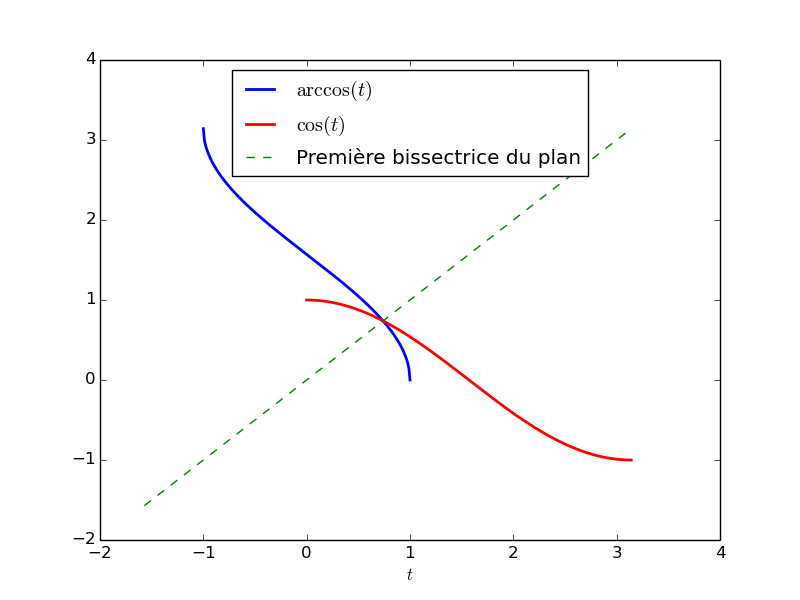
\includegraphics[scale = 0.7]{ex_avance}
%    \caption{Graphes des fonctions $\arccos$ et $\cos$}
%    \label{fig:ex_avance}
%  \end{center}
%\end{figure}  


